\fancyhead[LE,RO]{pK meghatározása vezetés mérésével -- ,,PKVEZ''}
\fancyhead[LO,RE]{\thesection}
\fancyfoot[LE,RO]{\thepage}
\fancyfoot[RE,LO]{\emph{Fizikai Kémia gyakorlatok gyógyszerész hallgatóknak}}

\setcounter{section}{7}
\section{Gyengesav disszociációs állandójának meghatározása vezetés mérésével}
\subsection{Bevezetés}
Az elektromos ellenállás anyagi tulajdonság.
Ohm törvénye értelmében egy anyagon átfolyó elektromos áram erősége ($I$) és az áramot létrehozó feszültség ($U$) között egyenes arányosság van:

\begin{equation}
\label{eq:ohm}
	U
	=
	I
	\cdot
	R
\end{equation}

ahol az $R$ arányossági tényezőt az illető anyag ellenállásának nevezzük, mértékegysége az ohm ($\ohm$).
Fajlagos ellenálláson az 1 m hosszú, 1 m$^2$ (a gyakorlatban 1 mm$^2$) keresztmetszetű vezetőn az 1 amper intenzitású áram létrehozásához szükséges feszültség és az áram hányadosát értjük.

Az elektrokémiában több szempontból előnyös, ha a fenti mértékegységek reciprokait használjuk: az ellenállás reciprokát vezetésnek (mértékegysége a Siemens, S = 1/$\ohm$), a fajlagos ellenállás reciprokát fajlagos vezetésnek nevezzük.

Elektrolitok oldatainak fajlagos vezetésén ($\kappa$) az 1 cm távolságban, párhuzamos, 1-1 cm$^2$ felületű elsőrendű (inert fém, pl. arany vagy gyakrabban platina) vezetőből készült elektródok között elhelyezkedő folyadékkocka vezetését értjük, mértékegysége S $\cdot$ cm$^{-1}$.
A fajlagos vezetés függ az elektrolit anyagi minőségétől, koncentrációjától, valamint a hőmérséklettől.
Moláris fajlagos vezetésen ($\Lambda _m$) azt értjük, mikor 1 cm-re elhelyezkedő elektródok közé 1 mol elektrolitot helyezünk el és a vezetést a fal mentén arra merőlegesen mérjük.
Ez alapján

\begin{equation}
\label{eq:lambdam}
        \Lambda_m
        =
        \frac
		{\kappa 1000 }
		{c}
	=
	\kappa V
\end{equation}

ahol $c$ az oldat koncentrációja (mol$\cdot$dm$^{-3}$) és $V$ a hígítás.
A vezetés szoros kapcsolatban van az ionok mozgékonyságával: ha ugyanis a mérő elektródra feszültséget kapcsolunk, az elektrolitban ionvándorlás indul meg.
A vándorlás sebessége függ az elektromos térerő nagyságától, ezért a vándorlási sebességet 1 V/cm térerőre vonatkoztatjuk.
Az 1 V/cm térerő hatására másodpercenként megtett utat az ion relatív mozgékonyságának ($u$) nevezzük.
Mivel egy biner elektrolitban mind az anionok, mind a kationok hozzájárulnak a vezetéshez, a fajlagos vezetés koncentrációtól való megváltozását

\begin{equation}
\label{eq:kohlrausch2}
	\kappa
	=
	c
	F
	(z_a \nu _a u_k + z_k \nu _k u_k)
	/1000
\end{equation}

formában írhatjuk fel erős elektrolitok híg oldataira, ahol $z_a, z_k$: ionok töltésszáma; $\nu _a, \nu _a$: sztöchiometriai konstansok; $F$: Faraday állandó.

Gyengeelektrolitok vezetése

\begin{equation}
\label{eq:lambdam}
        \lambda_c
        =
        \alpha
	\lambda_0
\end{equation}

formában adható meg, ahol $\alpha$ a disszociáció foka, $\lambda _0$ a végtelen hígítású oldat vezetése.
Ha a gyengeelektrolit koncentrációja kicsi, az ionmozgékonyságok csak a hőmérséklettől függenek, a koncentrációtól nem.
Egy AH gyengesav disszociációs állandója ($K_d$) kiszámítható a koncentráció és a disszociáció fokának ismeretében

\begin{equation}
\label{eq:kd}
        K_d
        =
        \frac{\alpha^2 c}{1-\alpha}
\end{equation}

Érdemes megjegyezni azonban, hogy a disszociációs állandó adott hőmérsékleten függ - a Debye-Hückel elmélet alapján - a közeg permittivitásától is.
Ha a \ref{eq:kd} egyenlet $\alpha$-ra rendezett alakját behelyettesítjük ez utóbbi egyenletbe, a gyengeelektrolitok disszociációjára Ostwald által megállapított összefüggéshez jutunk:

\begin{equation}
\label{eq:ostwald}
        K_d
        =
        \frac{\lambda_c^2 c}{\lambda_0^2 - \lambda_0\lambda_c}
\end{equation}

A disszociációs állandó értékét tehát vezetésméréssel meghatározhatjuk. 
$\lambda_c$ közvetlenül mérhető, míg $\lambda_0$ értékét az alábbiak szerint határozhatjuk meg:
A \ref{eq:ostwald} egyenlet átrendezésével

\begin{equation}
\label{eq:ostwald2}
        \frac{1}{\lambda_c}
        =
	\lambda_c
	c
	\frac{1}{K_d \lambda_0^2}
	+\frac{1}{\lambda_0}
\end{equation}

kifejezést kapjuk.
Ha ábrázoljuk $1/\lambda_c$-t $\lambda_c c$, azaz $\kappa$ függvényében, egyenest kapunk, melynek tengelymetszete $1/\lambda_0$. $\lambda_c$ és $\lambda_0$ ismeretében pedig $K_d$ értéke már kiszámítható.
A mérések kivitelezésekor a következőket kell figyelembe vennünk:
\begin{enumerate}[(a)]
\item Az oldat mért vezetéséhez az oldott anyag mellett az oldószer is hozzájárul.
Híg oldatok esetén ezért külön méréssel meghatározzuk az oldószer vezetését ($G_{\text{oldószer}}$) és ezt az értéket levonjuk az oldat esetében mért vezetés értékéből.

\item Az újabban használatos elektródok geometriája és elrendezésük eltérnek a fajlagos vezetés definíció szerinti meghatározásánál leírtaktól, ezért a mérőelektródot kalibrálni kell.
Az eltérés a mérést nem befolyásolja, mivel az eltérés az úgynevezett cellaállandó - mint kalibrációs paraméter - segítségével figyelembe vehető.
A cellaállandó (jele $C$, egysége m$^{-1}$ vagy cm$^{-1}$) megmutatja egy ismert fajlagos vezetésű oldat ($\kappa_{ref}$) és az adott mérőcellával ezen oldaton mért vezetés ($G_{\text{mért}}$) közötti kapcsolatot:

\begin{equation}
\label{eq:c}
	C
	=
	\kappa_{\text{ref}}/G_{\text{mért}}
\end{equation}

\end{enumerate}

Ezek alapján az oldat hozzájárulását a vezetéshez a következőképpen kapjuk meg: $\kappa_{\text{korr}} = (G_{\text{oldat}} - G_{\text{oldószer}})C$,
ahol $\kappa_{\text{korr}}$ az oldatnak a cellaállandóval és az oldószer fajlagos vezetésével korrigált értéke, $C$ a cellaállandó (nem tévesztendő össze a koncentrációval, melyet $c$-vel jelölünk).
Ezek alapján a gyengesav oldat moláris vezetése:

\begin{equation}
\label{eq:c}
        \lambda
        =
        \kappa_{korr}
	V
\end{equation}

ahol V a hígítás.

\begin{figure}
\centering
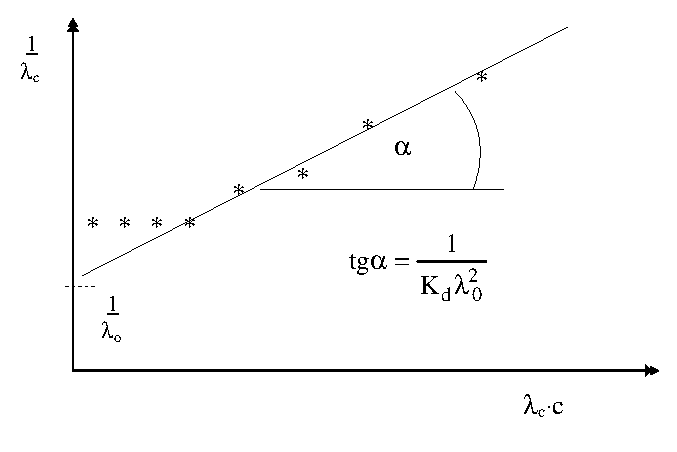
\includegraphics{lambda0.eps}
\caption{Végtelen higítású oldat vezetésének ($\lambda_0$) meghatározása.}
\label{fig:}
\end{figure}

\subsection{A gyakorlat leírása}

A konduktométer harangelektródját többször (4 - 5) öblítsük át desztillált vízzel majd kis részlet 1 $\upmu$ S/cm-nél kisebb fajlagos vezetésű vízzel, melyet külön edényben a technikustól kell kérni.
A gyakorlatvezető által kijelölt alkohollal (metanol, etanol vagy propanol) készítsünk 20 v/v\%-os oldatot.
A kijelölt 1 mol$\cdot$dm$^{-3}$ koncentrációjú gyengesav törzsoldatából pipettázzunk két száraz 100 cm$^3$-es mérőlombikba 2.00 cm$^3$-t, majd töltsük jelre az első lombikot vezetőképességi vízzel, a másikat a 20\%-os alkohol oldattal.
A mérést mérőhengerben végezzük.

Töltsük először a vizes hígítású oldatot a mérőedénybe, és mérjük meg a vezetését.
Ezután 25 cm$^3$-t pipettázzunk ki az oldatból és 50 cm$^3$-es mérőlombikban hígítsuk kétszeresére.
Az elektród gondos leöblítése után mérjük ezen oldat vezetését is.
Az oldat vezetését leghelyesebb úgy meghatározni, hogy az elektród bemerítésétől 5 percen át 30-60 másodpercenként észleljük és feljegyezzük a cellában jelentkező vezetés értékeket.
A kétszeres hígítást még 3-4-szer megismételjük, minden alkalommal mérve a vezetést.

Ismételjük meg a méréseket az alkoholt tartalmazó oldatokkal is úgy, hogy a hígítások során bidesztillált víz helyett a mérőlombikot az alkoholos oldattal töltjük mindig jelre.

A mérőcellában egy-egy oldatot legalább 25 percig kell termosztálni.
A rendelkezésre álló idő rövidsége miatt a legcélszerűbb, ha a sorozat következő, már meghígított tagját főzőpohárban előre a termosztátba helyezzük, így csökkentve a két mérés közti várakozási időt.

Végül mérjük meg mind a hígításokhoz használt vezetőképességi víz, mind az alkohol oldat vezetését, melyekkel mérési eredményeinket korrigálnunk kell.
Ezután határozzuk meg 0.1 és 0.01 M KCl oldatok felhasználásával a cellaállandó értékét úgy, hogy cellakonstansként a két mérésből számolt értékek átlagát fogadjuk el.

\subsection{A mérési eredmények kiértékelése}

\begin{enumerate}
\item Számítsuk ki a cellaállandó értékét.
A mérési eredményeket a vizes és az alkoholos sorozatnál is foglaljuk táblázatba:

\begin{table}[!h]
\centering
\begin{tabular}{|c|c|c|c|c|c|c|c|}
\hline
c (mol $\cdot$ dm$^{-3}$) & G$_{\text{mért}}$ & $\kappa_{\text{korr}}$ (S $\cdot$ cm$^{-1}$) & $\lambda_c$ & $1/\lambda_c$ & $\lambda_c c$ & $\alpha$ & $K_d$ \\
\hline
... & ... & ... & ... & ... & ... & ... & ... \\
\end{tabular}
\label{table:vez}
\end{table}

\item Határozzuk meg grafikusan $\lambda_0$ értékét, $\lambda_c$ és $\lambda_0$ ismeretében pedig minden koncentrációra számítsuk ki $\alpha$ és $K_d$ értékeit.

\end{enumerate}

A \ref{fig:vez}. ábra egy vezetőképesség mérésére szolgáló cella felépítését mutatja.
A mérendő oldatba egy geometriailag jól definiált, indifferens elektródpárt merítünk és az ezen létrejövő feszültségesést mérjük.
A konduktometria gyakorlatban az elektrolízis, ill. az elektromos polarizáció csökkentése, ill. kiküszöbölése érdekében váltóárammal végezzük a mérést.

\begin{figure}
\centering
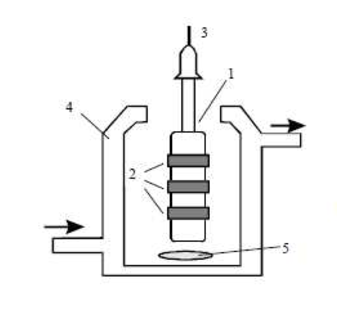
\includegraphics{cond.eps}
\caption{Vezetőképesség mérésére szolgáló cella felépítése. 1 - harangelektród, 2 - Pt korommal bevont gyűrűk, 3 - elektromos elvezetés, 4 - kettős falú temperálható edény, 5 - mágneses keverő.}
\label{fig:vez}
\end{figure}


